\section{Введение}
Нуклеосинтезом называют совокупность протекающих в естественных условиях ядерных процессов, приводящих к образованию атомных ядер. Исследование механизмов нуклеосинтеза является актуальной задачей современной физики, так как они определяют распространенность ядер химических элементов во Вселенной и играют важную роль в астрофизике. Нуклеосинтез сопровождает эволюцию Вселенной с самого ее рождения. В первичном, дозвездном нуклеосинтезе, начавшемся уже в первые секунды после Большого взрыва, стали возникать легчайшие ядра, изотопы водорода и гелия. Наблюдаемое сегодня подавляющее преобладание ядер ${}^1$H и ${}^4$He сложилось именно за счет дозвездного нуклеосинтеза. В звездном нуклеосинтезе, начавшемся приблизительно через 1 млрд лет с появлением первых звезд, в результате стадий термоядерного горения, чередующихся со стадиями гравитационного сжатия, образуются ядра химических элементов вплоть до железа. Термоядерное горение обеспечивает светимость звезды и сдерживает ее сжатие.

\begin{figure}[!b]
  \centering
  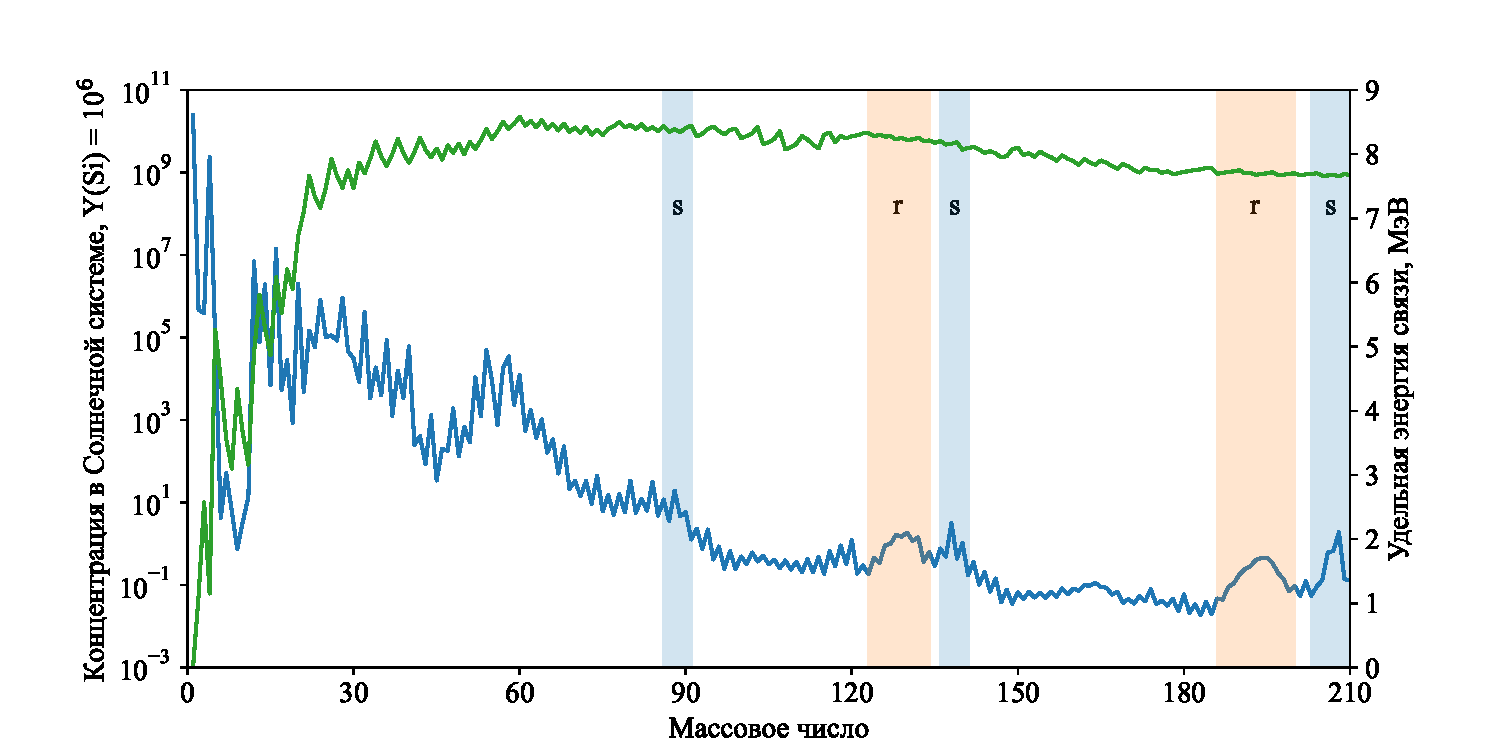
\includegraphics[width=0.8\textwidth]{pics/lodders_vs_ame.pdf}
  \caption{Массовое распределение ядер в Солнечной системе по данным~\cite{lodders2003}, масса изотопов Si принята равной $10^6$. Оранжевым отмечены пики $r$-процесса, синим --- пики $s$-процесса (согласно~\cite{cowan2021}).}
  \label{fig:lodders_vs_ame}
\end{figure}

Астрофизическим $r$-процессом, или процессом быстрого нейтронного захвата, называется механизм нуклеосинтеза, в ходе которого исходное ядро поглощает большое число нейтронов и, оказавшись в области нейтронного избытка, испытывает слабые распады. В результате масса ядра увеличивается за счет поглощенных нейтронов, а $\beta^-$-распады приводят к образованию химического элемента с большим зарядовым числом. В $r$-процессе скорости нейтронного захвата на порядки превышают скорости $\beta^-$-распадов, что обеспечивает стремительный набор массы и значительное смещение в область нейтронного избытка. Для достижения необходимой интенсивности поглощения нейтронов требуется высокая плотность их потока, около 150 нейтронов на одно зародышевое ядро, и температуры вещества свыше 1~ГК. Такие экстремальные условия могут реализовавываться при катастрофических явлениях: взрывах сверхновых, слияниях двух нейтронных звезд, слияниях нейтронной звезды и черной дыры. 

По современным представлениям, именно $r$-процесс обеспечивает возникновение основной массы ядер химических элементов тяжелее железа во Вселенной. Синтез более легких ядер обеспечивается термоядерным горением звездного вещества, но, как известно, им невозможно объяснить возникновение химических элементов за так называемым <<железным пиком>>, максимумом зависимости удельной энергии связи от массового числа. Процесс медленного нейтронного захвата, или $s$-процесс, отличающийся от $r$-процесса значительно меньшей интенсивностью поглощения нейтронов и, соответственно, характерными временами порядка сотен лет, требует не столь исключительных астрофизических условий и обеспечивает образование ядер вблизи долины стабильности вплоть до свинца и висмута. Однако $s$-процессом нельзя объяснить существование более тяжелых ядер, а также нейтроноизбыточных изотопов, слишком удаленных от долины стабильности. Некоторое количество обойденных протоноизбыточных изотопов возникает в $p$-процессе, механизме взровного нуклеосинтеза, представляющем собой последовательности фотоядерных реакций и поглощений заряженных частиц. Однако выходы $p$-процесса малы по сравнению с $s$- и $r$-процессами. Кроме того, для синтеза $p$-изотопов требуется наличие достаточно тяжелых стабильных ядер, достаточное число которых может образоваться только в результате процессов нейтронного захвата. 

На рис.~\ref{fig:lodders_vs_ame} представленно массовое распределение ядер в Солнечной системе, построенное по данным~\cite{lodders2003}. Виден избыток легчайших изотопов с $A \leq 4$, родившихся в первичном нуклеосинтезе, за которым следует минимум, соответствующий изотопам Li, Be и B. С массового числа 12 начинается область ядер, рождающихся в основном за счет термоядерного горения звездного вещества, в частности, pp- и CNO-циклов. Видно, что начиная с массовых чисел $54 - 58$, соответствующих <<железному пику>>, начинается существенное снижение концентраций изотопов. В области более тяжелых ядер нуклеосинтез целиком обеспечивается $s$- и $r$-процессами. На рис.~\ref{fig:lodders_vs_ame} отмечены характерные пики, соответствующие магическим числам нейтронов 50, 82 и 126, что является указанием на высокий вклад процессов нейтронного захвата в нуклеисинтез. Более узкие пики образуются благодаря $s$-процессу, который протекает вблизи долины стабильности, в то время как $r$-процесс рождает сверх-нейтроноизбыточные ядра. Для таких экзотических изотопов могут преобладать уже не $\beta^-$-распады, протекающие без потери массы, а слабые распады с вылетом нейтронов, что приводит к размыванию и смещению пика $r$-процесса в область меньших масс.

Основным методом исследования $r$-процесса и эволюции астрофизических ядерных систем в целом является математическое моделирование, сводящееся к решению системы обыкновенных дифференциальных уравнений (ОДУ) большой размерности. Численное интегрирование таких задач само по себе представляет существенные трудности. Входными параметрами такой системы ОДУ являются температуры и плотности среды, определяемые астрофизическим сценарием, и свойства участвующих в $r$-процессе реакций и ядер. Так как путь $r$-процесса лежит в основном в области экзотических нейтроноизбыточных ядер, экспериментальное изучение которых в лабораторных условиях представляется невозможным, их характеристики приходится получать при помощи теоретических ядерных моделей. При этом различные ядерные модели могут давать существенно разные результаты для экзотических изотопов, например, при расчете энергий связи~\cite{sobiczewski2018}. Неопределенности входных ядерных данных могут существенно сказываться на результатах расчета $r$-процесса, на что указывается, например, в статье~\cite{goriely2001}.

Целью настоящей работы является определение чувствительности модели $r$-процесса к неопределенностям расчета масс нейтроноизбыточных ядер. Для этого нами были рассмотрены результаты трех расчетов масс нейтроноизбыточных ядер, выполненных при помощи различных ядерных моделей. При помощи этих теоретических значений масс были проведены расчеты сечений реакций нейтронного захвата и построены библиотеки астрофизических ядерных реакций, в которых учтено изменение границ области существования ядер в зависимости от используемой массовой модели. Уделено также внимание $\beta^-$-распадам, играющим большую роль в $r$-процессе. Полученные библиотеки реакций использованы при симуляции $r$-процесса в реалистичном астрофизическом сценарии слияния двух нейтронных звезд. Различия результирующих массовых распределений $r$-изотопов позволили оценить влияние неопределенностей теоретических значений масс нейтроноизбыточных ядер на моделирование $r$-процесса.
